\documentclass[11pt,a4paper]{article}

\usepackage[utf8]{inputenc}
\usepackage[T1]{fontenc}
\usepackage[margin=1in]{geometry}
\usepackage[table]{xcolor}
\usepackage[most]{tcolorbox}
\usepackage{hyperref}
\usepackage{tabularx}
\usepackage{booktabs}
\usepackage{tikz}
\usepackage{fancyhdr}
\usepackage{fontawesome5}
\usepackage{amsmath}
\usepackage{graphicx}
\usepackage{float}

% --- Premium Typography & Spacing ---
\usepackage{mathpazo}
\usepackage{setspace}
\setstretch{1.15}

% --- Premium Section Headings ---
\usepackage{titlesec}
\titleformat{\section}
  {\normalfont\Large\bfseries\color{dpiblue}}{\thesection}{1em}{}[{\color{dpicloud}\vspace{0.2cm}\titlerule[1pt]}]
\titleformat{\subsection}
  {\normalfont\large\bfseries\color{dpiteal}}{\thesubsection}{1em}{}

% --- Premium Hyperlinks ---
\hypersetup{
    colorlinks=true,
    linkcolor=dpiblue,
    filecolor=dpiblue,      
    urlcolor=dpiteal,
    citecolor=dpiblue
}

% Custom Header Style
\pagestyle{fancy}
\setlength{\headheight}{25pt}
\fancyhf{}
\fancyhead[L]{\raisebox{-0.2\height}{
\includegraphics[height=15pt]{logo.png}}\hspace{0.2cm}\textbf{\color{dpiblue} DPI-LS Framework}}
\fancyhead[R]{\color{dpiblue} Measuring Productivity (P)}
\fancyfoot[C]{\color{dpiblue}\textbf{Page \thepage}}
\renewcommand{\headrulewidth}{1pt}
\renewcommand{\headrule}{\hbox to\headwidth{\color{dpiblue}\leaders\hrule height \headrulewidth\hfill}}
\usetikzlibrary{shapes.geometric, arrows.meta, positioning, calc, backgrounds, fit, trees, mindmap, matrix, shadows}

% Define DPI-LS Brand Colors
\definecolor{dpiblue}{HTML}{2b3a67}
\definecolor{dpigreen}{HTML}{498467}
\definecolor{dpired}{HTML}{b0413e}
\definecolor{dpilight}{HTML}{e5f9e0}
\definecolor{dpicloud}{HTML}{f4a261}
\definecolor{dpiteal}{HTML}{318281}

% Define Custom GitHub-Style Alerts
\newtcolorbox{dpinote}[1][]{enhanced, colback=blue!5!white, colframe=dpiblue, title={\textbf{\faInfoCircle\ NOTE}}, fonttitle=\bfseries, attach boxed title to top left={xshift=5mm,yshift=-2mm}, #1}
\newtcolorbox{dpiimportant}[1][]{enhanced, colback=red!5!white, colframe=dpired, title={\textbf{\faExclamationTriangle\ IMPORTANT}}, fonttitle=\bfseries, attach boxed title to top left={xshift=5mm,yshift=-2mm}, #1}
\newtcolorbox{dpitip}[1][]{enhanced, colback=dpigreen!5!white, colframe=dpigreen, boxrule=0.5pt, leftrule=3pt, sharp corners, #1}

\begin{document}

\begin{titlepage}
    \pagecolor{dpiblue}
    \color{white}
    \begin{center}
        \vspace*{1.5cm}
        
\includegraphics[width=6cm]{logo.png} \\[1.5cm]
        
        {\Huge \textbf{Measuring Productivity}} \\[0.7cm]
        {\LARGE \textbf{Guide for the DPI-LS Project}}
        
        \vspace{2cm}
        
        {\color{dpicloud}\rule{0.5\textwidth}{1.5pt}}
        
        \vspace{2cm}
        
        {\Large \textit{Digital Performance Index --- Productivity Dimension (P)}} \\[1cm]
        
        {\large AI Task Completion, Throughput \& Hyper-Scaling}
        
        \vfill
        
        % Stylish Geometric Cover Overlay
        \begin{tikzpicture}[remember picture, overlay]
            \fill[white, opacity=0.05] (current page.north east) circle (5cm);
            \fill[white, opacity=0.05] (current page.south west) circle (7cm);
            \fill[dpiteal, opacity=0.1] (current page.south east) circle (9cm);
            
            % Giant faded icon in the center as a watermark
            \node[font=\fontsize{150}{150}\selectfont, text=white, opacity=0.03] at (current page.center) {\faRocket};
        \end{tikzpicture}
        
        \renewcommand{\arraystretch}{1.3}
        \begin{tabular}{rl}
            \textbf{Framework:} & Digital Performance Index (DPI-LS) \\
            \textbf{Dimension:} & Productivity (P) --- Weight: 15\% \\
            \textbf{Version:} & 1.0 (Extended Enterprise Edition) \\
            \textbf{Status:} & Architectural Reference \\
        \end{tabular}
        
        \vspace{2cm}
        
        {\color{dpicloud}\rule{0.5\textwidth}{1pt}} \\[0.5cm]
        
        {\large DPI-LS Architecture Team}
        
        \vspace{0.3cm}
        {\normalsize Document Developed by \textbf{Malkapurapu Sivamanikanta}}
        
        \vspace*{1cm}
    \end{center}
\end{titlepage}
\pagecolor{white}
\color{black}

\tableofcontents
\newpage

% ---------------------------------------------------------
% 1. EXECUTIVE SUMMARY & INTRODUCTION
% ---------------------------------------------------------
\section{Executive Summary \& Introduction}

\begin{dpinote}
The \textbf{Digital Performance Index (DPI-LS)} framework quantifies AI agent performance across 7 distinct dimensions. Within this framework, the \textbf{Productivity (P)} dimension measures an agent's sheer output volume compared to a deterministic human baseline.
\end{dpinote}

Autonomous AI Agents operate at speeds incomprehensible to human operators. A single AutoGPT or LangGraph instance deployed on highly concurrent Kubernetes pods can resolve thousands of Jira tickets or analyze millions of log lines in the time it takes a human to open their laptop. 

However, measuring sheer volume is not enough. If an agent completes 10,000 tasks, but the mathematical scoring model allows the Productivity metric to scale infinitely, the final composite DPI-LS score would break, yielding scores of $50,000\%$ and completely masking failures in Quality, Risk, and Cost.

This technical architectural reference outlines the guidelines for capturing \textbf{Productivity (P)}, detailing the $1.0$ boundary cap limit, and illustrating how orchestration layers pass telemetry into the DPI-LS Engine to evaluate true autonomous throughput.

\vspace{0.5cm}
\hrule
\vspace{1cm}

% ---------------------------------------------------------
% 2. PRODUCTIVITY STRATEGY MIND MAP
% ---------------------------------------------------------
\section{Productivity Strategy Mind Map}

The following mind map defines the core operational pillars of AI Agent Productivity monitored within the DPI-LS framework.

\vspace{0.5cm}
\begin{center}
\resizebox{0.9\textwidth}{!}{
\begin{tikzpicture}[
  mindmap,
  every node/.style={concept, execute at begin node=\hskip0pt, drop shadow},
  root concept/.append style={concept color=dpiblue, fill=dpiblue, line width=1ex, text=white, font=\large\bfseries},
  level 1 concept/.append style={font=\small\bfseries, level distance=5.5cm, text=white},
  level 2 concept/.append style={font=\footnotesize, level distance=3cm, text=black},
  grow cyclic
]
\node[root concept] {AI Agent \\ Productivity}
  child[concept color=dpigreen, sibling angle=90] { node {Task \\ Throughput}
    child[sibling angle=45] { node[fill=white] {Completed \\ Assignments} }
    child[sibling angle=45] { node[fill=white] {Resolution \\ Velocity} }
  }
  child[concept color=dpicloud, sibling angle=90] { node {Hyper-Scaling \\ \& Concurrency}
    child[sibling angle=45] { node[fill=white] {Parallel \\ Threads} }
    child[sibling angle=45] { node[fill=white] {Stateless \\ Execution} }
  }
  child[concept color=dpired, sibling angle=90] { node {Blockers \& \\ Failure States}
    child[sibling angle=45] { node[fill=white] {Permission \\ Denials} }
    child[sibling angle=45] { node[fill=white] {Pending \\ Approvals} }
  }
  child[concept color=dpiteal, sibling angle=90] { node {Human \\ Baselines}
    child[sibling angle=45] { node[fill=white] {SME Manual \\ Output} }
    child[sibling angle=45] { node[fill=white] {Normalization \\ Factors} }
  };
\end{tikzpicture}
}
\end{center}
\vspace{0.5cm}

\newpage

% ---------------------------------------------------------
% 3. THE MATHEMATICS OF PRODUCTIVITY
% ---------------------------------------------------------
\section{The Mathematics of Productivity}

The Productivity dimension provides a normalized score indicating how effectively an agent produces output relative to human workers. Productivity carries a weighting of \textbf{15\% (0.15)} on the final composite DPI-LS score.

\begin{dpiimportant}
\textbf{Formula:} $P = \min\left(1.0, \frac{\text{AI Tasks} \times \text{Normalization Factor}}{\text{Human Baseline}}\right)$
\end{dpiimportant}

\begin{itemize}
    \item \textbf{\color{dpiblue}\faRobot\ AI Tasks Completed:} The raw integer of tasks successfully resolved by the agent in the given time period (e.g., 500 tickets).
    \item \textbf{\color{dpiteal}\faUserTie\ Human Baseline:} The predetermined integer of tasks a human Subject Matter Expert (SME) completes in the exact same time period (e.g., 10 tickets).
    \item \textbf{\color{dpigreen}\faBalanceScale\ Normalization Factor:} A static configuration float used to tune agents with extremely disparate workflows. Default is $1.0$.
\end{itemize}

\subsection{The 1.0 Boundary Cap}

The most critical element of the Productivity equation is the \texttt{min(1.0, X)} bounding logic. Because agents operate at cloud-scale, an agent might complete $10,000$ tasks while the human baseline is only $10$. This results in a raw ratio of $1,000.0$.

If the DPI-LS Engine accepted $1,000.0$ as a valid sub-metric, applying the 15\% weighting ($1000.0 \times 0.15$) would yield a composite score addition of $+150.0$. This would instantly destroy the integrity of the index, masking terrible Quality or Risk scores by overwhelming the math with sheer volume.

Therefore, the engine strictly caps $P$ at $1.0$ (100\%). The goal is to prove the agent is \textit{at least as productive} as a human, not to break the scoring system.

\subsection{Deep Math: Throughput Vectors \& Complexity Weighting}

While the base formula provides a simple ratio, enterprise environments rarely process identical tasks. The \textbf{Normalization Factor} in the DPI-LS Engine acts as an aggregate complexity multiplier, transforming raw task counts into a \textit{Throughput Vector}.

Let $T = \{t_1, t_2, \dots, t_n\}$ be the set of $n$ tasks completed by the agent in a given period.
Each task $t_i$ has an associated complexity weight $w_i \in (0, 5]$.

The effective AI Output, $\hat{O}_{\text{AI}}$, is calculated as the sum of all task complexity weights:
\[
\hat{O}_{\text{AI}} = \sum_{i=1}^{n} w_i
\]

The Human Baseline, $B_H$, is similarly defined by the expected complexity throughput of a Subject Matter Expert in the same period.

The Productivity score $P$ utilizes a bounded normalization function to ensure the final metric $P \in [0, 1]$:
\[
P = f(\hat{O}_{\text{AI}}, B_H) = \begin{cases} 
      1.0 & \text{if } \hat{O}_{\text{AI}} \geq B_H \\
      \frac{\hat{O}_{\text{AI}}}{B_H} & \text{if } \hat{O}_{\text{AI}} < B_H 
   \end{cases}
\]

This piecewise function mathematically guarantees that hyper-scaling an agent to process 1,000,000 tasks ($ \hat{O}_{\text{AI}} \gg B_H $) does not mathematically overwhelm the composite $0.15$ dimension weight. The Heaviside step limits the ceiling strictly at $1.0$, preventing index distortion.

\subsubsection{Deriving the Normalization Factor ($\gamma$)}

The Normalization Factor (denoted as $\gamma$) is not an arbitrary constant; it is a mathematically derived scalar representing the relative complexity density of an AI task compared to a standard human task.

Let $C$ represent a function that calculates the sheer computational complexity of a task based on three distinct dimensions:
\begin{itemize}
    \item $t_d$: \textbf{Token Depth} (Context window utilization in tokens).
    \item $a_c$: \textbf{API Call Count} (Number of external system interactions).
    \item $d_b$: \textbf{Decision Branches} (Cyclomatic complexity of the execution graph).
\end{itemize}

For any given task $i$, its intrinsic complexity $C_i$ is given by a weighted linear combination:
\[
C_i = \alpha_1(t_{d, i}) + \alpha_2(a_{c, i}) + \alpha_3(d_{b, i})
\]
where $\alpha_1, \alpha_2, \alpha_3$ are predetermined coefficient weights tuning the impact of each variable.

The overarching Normalization Factor $\gamma$ for an agent deployed on a specific queue is then the ratio of the expected value of AI task complexity $E[C_{\text{AI}}]$ to the expected value of Human task complexity $E[C_{\text{Human}}]$:
\[
\gamma = \frac{E[C_{\text{AI}}]}{E[C_{\text{Human}}]} = \frac{\frac{1}{N_{\text{AI}}} \sum_{i=1}^{N_{\text{AI}}} C_{\text{AI}, i}}{\frac{1}{N_{\text{Human}}} \sum_{j=1}^{N_{\text{Human}}} C_{\text{Human}, j}}
\]

\begin{dpiimportant}
If an agent is resolving basic password resets, its $E[C_{\text{AI}}]$ is low. If a human is resolving tier-3 database corruptions, their $E[C_{\text{Human}}]$ is extremely high. In this scenario, $\gamma < 1.0$ (e.g., $\gamma = 0.2$), meaning the agent must complete \textbf{5 times as many tasks} just to equate to one human task.
\end{dpiimportant}
% Masterclass example will go at the end of the section.

% Replaced Queue Theory with a simple spacer before the Masterclass
\vspace{0.5cm}

\newpage
\section{Mathematical Masterclass: End-to-End Score Calculation}

The following masterclass walks through the exact end-to-end mathematical pipeline used by the DPI-LS engine to calculate an agent's final Productivity score. We break this down into 6 comprehensive phases, detailing every arithmetic step and explaining the \textit{business rationale} behind the math.

\vspace{0.5cm}

% ---------------- PHASE 1 ----------------
\subsection{Phase 1: Define the Complexity Constants}

Before we can compare an AI agent to a human, we must define what makes a task "complex". A task that requires reading 100,000 tokens of context is inherently harder than a task that requires reading 100 tokens. 

The Enterprise Architecture board defines the intrinsic weighting constants for the complexity formula $C_i = \alpha_1(t_d) + \alpha_2(a_c) + \alpha_3(d_b)$.

\begin{tcolorbox}[enhanced, colback=dpicloud!5!white, colframe=dpiblue, title={\textbf{Phase 1: Architecture Constants}}, fonttitle=\bfseries]
\begin{itemize}
    \item \textbf{Token Depth Weight ($\alpha_1$):} $0.001$ 
    \begin{itemize}
        \item \textit{Rationale:} Reading text is computationally cheap but contextually heavy. We assign $0.001$ points per token processed.
    \end{itemize}
    \item \textbf{API Call Weight ($\alpha_2$):} $2.5$ 
    \begin{itemize}
        \item \textit{Rationale:} External API calls introduce latency, auth complexity, and failure risks. Each call adds a heavy $2.5$ points.
    \end{itemize}
    \item \textbf{Decision Branch Weight ($\alpha_3$):} $5.0$ 
    \begin{itemize}
        \item \textit{Rationale:} Cyclomatic complexity (if/else logic) is the hardest thing for LLMs to navigate. Each branch adds a massive $5.0$ points.
    \end{itemize}
\end{itemize}
\end{tcolorbox}

\newpage

% ---------------- PHASE 2 ----------------
\subsection{Phase 2: Calculate the Expected AI Task Complexity ($E[C_{\text{AI}}]$)}

Assume the AI agent processes complex infrastructure provisioning tasks (e.g., spinning up Kubernetes clusters via Terraform). Over a sample of $N_{\text{AI}} = 1,000$ tasks, we pull the telemetry to find the mean task metrics.

\vspace{0.3cm}
\textbf{Raw AI Telemetry Averages:}
\begin{itemize}
    \item Average Token Depth ($E[t_d]$): $60,000$ tokens per task.
    \item Average API Calls ($E[a_c]$): $16$ calls per task.
    \item Average Decision Branches ($E[d_b]$): $4$ logical branches per task.
\end{itemize}

\begin{tcolorbox}[enhanced, colback=dpicloud!5!white, colframe=dpigreen, title={\textbf{Phase 2: Step-by-Step AI Arithmetic}}, fonttitle=\bfseries]
We multiply the raw telemetry by the Phase 1 constants:
\vspace{0.2cm}
\begin{itemize}
    \item \textbf{Token Load Calculation:} 
    \[ 60,000 \text{ tokens} \times 0.001 = \mathbf{60.0} \text{ complexity points} \]
    \item \textbf{API Load Calculation:} 
    \[ 16 \text{ calls} \times 2.5 = \mathbf{40.0} \text{ complexity points} \]
    \item \textbf{Branch Load Calculation:} 
    \[ 4 \text{ branches} \times 5.0 = \mathbf{20.0} \text{ complexity points} \]
\end{itemize}

\vspace{0.2cm}
\textbf{Final Expected AI Complexity:}
\[
E[C_{\text{AI}}] = 60.0 \text{ (Tokens)} + 40.0 \text{ (APIs)} + 20.0 \text{ (Branches)} = \mathbf{120.0}
\]
The average task this AI agent completes has a mathematical "weight" of $120.0$.
\end{tcolorbox}

\newpage

% ---------------- PHASE 3 ----------------
\subsection{Phase 3: Calculate the Expected Human Task Complexity ($E[C_{\text{Human}}]$)}

Now we must define the baseline. Assume a Human Subject Matter Expert (SME) resolves standard baseline IT tickets. We translate their workflow into the same framework to find their expected complexity.

\vspace{0.3cm}
\textbf{Raw Human Telemetry Averages:}
\begin{itemize}
    \item Average Equivalent Token Depth ($E[t_d]$): $40,000$ tokens.
    \item Average API Calls ($E[a_c]$): $12$ calls (clicks/queries).
    \item Average Decision Branches ($E[d_b]$): $6$ logical branches.
\end{itemize}

\begin{tcolorbox}[enhanced, colback=dpicloud!5!white, colframe=dpiteal, title={\textbf{Phase 3: Step-by-Step Human Arithmetic}}, fonttitle=\bfseries]
We multiply the raw telemetry by the Phase 1 constants:
\vspace{0.2cm}
\begin{itemize}
    \item \textbf{Token Load Calculation:} 
    \[ 40,000 \text{ tokens} \times 0.001 = \mathbf{40.0} \text{ complexity points} \]
    \item \textbf{API Load Calculation:} 
    \[ 12 \text{ calls} \times 2.5 = \mathbf{30.0} \text{ complexity points} \]
    \item \textbf{Branch Load Calculation:} 
    \[ 6 \text{ branches} \times 5.0 = \mathbf{30.0} \text{ complexity points} \]
\end{itemize}

\vspace{0.2cm}
\textbf{Final Expected Human Complexity:}
\[
E[C_{\text{Human}}] = 40.0 \text{ (Tokens)} + 30.0 \text{ (APIs)} + 30.0 \text{ (Branches)} = \mathbf{100.0}
\]
The average task the human baseline completes has a mathematical "weight" of $100.0$.
\end{tcolorbox}

\newpage

% ---------------- PHASE 4 ----------------
\subsection{Phase 4: Derive the Normalization Factor ($\gamma$)}

We now have the mathematical proof that the agent is doing harder work than the human. The agent is scoring $120.0$ points per task, while the human is scoring $100.0$ points per task. 

To make a fair comparison in Productivity, we calculate the Normalization Factor multiplier.

\begin{tcolorbox}[enhanced, colback=orange!5!white, colframe=orange, title={\textbf{Phase 4: The $\gamma$ Ratio Calculation}}, fonttitle=\bfseries]
The engine divides the AI complexity by the Human complexity:
\[
\gamma = \frac{E[C_{\text{AI}}]}{E[C_{\text{Human}}]} = \frac{120.0}{100.0} = \mathbf{1.20}
\]
\textbf{Business Meaning:} Every $1$ task the AI completes is mathematically equivalent to $1.20$ human tasks due to the increased token depth and API overhead.
\end{tcolorbox}

\vspace{0.5cm}

% ---------------- PHASE 5 ----------------
\subsection{Phase 5: Calculate the Throughput Ratio}

With the $\gamma$ multiplier locked in at $1.20$, we can finally look at the raw Volume (how many tasks were actually finished today).

\begin{itemize}
    \item \textbf{Human Baseline Volume ($B_H$):} The human SME finished \textbf{40} standard tickets today.
    \item \textbf{AI Agent Volume ($n$):} The AI agent finished \textbf{20} complex tickets today.
\end{itemize}

\begin{tcolorbox}[enhanced, colback=dpiblue!5!white, colframe=dpiblue, title={\textbf{Phase 5: Effective Output Calculation}}, fonttitle=\bfseries]
If we just looked at raw volume, the AI lost (20 vs 40). But we must apply the $\gamma$ multiplier to find the \textit{Effective Output} ($\hat{O}_{\text{AI}}$):
\[
\hat{O}_{\text{AI}} = n \times \gamma = 20 \text{ tasks} \times 1.20 = \mathbf{24.0} \text{ Effective Output}
\]
\textbf{Business Meaning:} By completing 20 highly complex tasks, the AI generated the equivalent productivity of 24 standard human tasks.
\end{tcolorbox}

\newpage

% ---------------- PHASE 6 ----------------
\subsection{Phase 6: Apply the Piecewise Bounding Function (Final Score)}

We have all the variables. The AI produced an effective output of $24.0$. The human baseline was $40.0$. We now run these values through the strict DPI-LS boundary function.

\begin{tcolorbox}[enhanced, colback=dpigreen!5!white, colframe=dpigreen, title={\textbf{Phase 6: The Bounding Cap}}, fonttitle=\bfseries]
To prevent infinite score inflation, the DPI-LS Engine strictly bounds the final Productivity score $P$:
\[
P = \min\left(1.0, \frac{\hat{O}_{\text{AI}}}{B_H}\right)
\]
\[
P = \min\left(1.0, \frac{24.0}{40.0}\right)
\]
\[
P = \min(1.0, 0.60) = \mathbf{0.60}
\]

\vspace{0.2cm}
\textbf{Final Masterclass Conclusion:} \\
The AI agent successfully processed highly complex tasks ($120.0$ complexity), yielding a $\gamma$ multiplier of $1.20$. However, it only managed to complete a raw volume of 20 tickets. 

Factoring in the $1.20$ complexity multiplier, its \textit{Effective Output} was mathematically raised to 24. 

When comparing this effective output of 24 against the human baseline of 40, the agent achieved a ratio of $0.60$. Because $0.60$ is below the $1.0$ maximum ceiling, the engine accepts it organically without applying a bounding cap. 

The agent earns a final Productivity dimension score of \textbf{0.60 (60\%)}.
\end{tcolorbox}

\vspace{0.5cm}

\subsection{Deep Math: Amdahl's Law in Concurrency Limits}

To achieve high Productivity scores, agents are often deployed in parallel (e.g., 500 concurrent LangGraph threads). However, \textbf{Amdahl's Law} dictates the strict mathematical ceiling of this approach when external APIs (like Jira or GitHub) rate-limit the agent, forcing sequential processing.

Let $S$ be the theoretical speedup of the agent swarm. Let $p$ be the proportion of the task that can be parallelized, and $c$ be the number of concurrent threads:
\[
S(c) = \frac{1}{(1-p) + \frac{p}{c}}
\]

If an agent task is 90\% parallelizable ($p=0.9$) but 10\% strictly sequential (e.g., waiting for an API lock), no amount of compute scaling will ever push the productivity speedup beyond a factor of $10x$, regardless of how many thousands of threads are provisioned. The DPI-LS engine tracks worker concurrency telemetry against $S(c)$ to flag \textbf{diminishing returns} in agent scaling.

\vspace{0.5cm}

\subsection{Business Math: The Widget Factory Analogy}

\begin{tcolorbox}[enhanced, colback=dpicloud!10!white, colframe=dpicloud, title={\textbf{\faLightbulb\ The Widget Factory Analogy}}, fonttitle=\bfseries\large, boxrule=1pt, arc=2mm, drop shadow]
To understand the baseline math, imagine you own a factory that builds widgets:

\vspace{0.2cm}
\begin{itemize}
    \item \textbf{\color{dpiblue}\faUserTie\ Human Output:} Your best human employee can assemble \textbf{10 widgets per day}. This is your baseline.
    \item \textbf{\color{dpigreen}\faRobot\ AI Output:} You install a robotic arm. On its first day, it builds \textbf{5 widgets} because it ran out of parts. Its Productivity score is $5 / 10 = \textbf{0.50 (50\%)}$.
    \item \textbf{\color{dpired}\faBalanceScale\ The Hyper-Scale Bounding:} The next day, you connect the robot to the main power grid. It builds \textbf{10,000 widgets}. The raw math is $10,000 / 10 = 1,000$. But you only \textit{needed} it to beat the human to get a perfect score. Thus, the engine caps the robot's Productivity score at exactly \textbf{1.0 (100\%)}.
\end{itemize}
\end{tcolorbox}

\newpage

\subsection{The Final P-Score Calculation Flow}

The diagram below illustrates the horizontal mathematical flow of data to calculate the final $P$ score, matching the exact 6-phase mathematical masterclass example.

\vspace{1cm}
\begin{center}
\resizebox{1.0\textwidth}{!}{
\begin{tikzpicture}[
    node distance=1.0cm and 0.5cm,
    incident/.style={rectangle, draw=dpiblue, fill=dpicloud!20, thick, text width=2.8cm, align=center, minimum height=1cm, rounded corners},
    critical/.style={rectangle, draw=orange, fill=orange!10, thick, text width=2.8cm, align=center, minimum height=1cm, rounded corners},
    arrow/.style={-{Stealth[scale=1.2]}, thick, dpiblue},
    result/.style={rectangle, draw=dpigreen, fill=dpilight, thick, text width=3.5cm, align=center, minimum height=1.5cm, rounded corners, drop shadow}
]

% Row 1: The Raw Input
\node[incident] (ai_comp) {AI Complexity\\$E[C_{\text{AI}}] = 120.0$};
\node[incident, right=1.5cm of ai_comp] (hu_comp) {Human Complexity\\$E[C_{\text{Human}}] = 100.0$};
\node[critical, right=1.5cm of hu_comp] (gamma) {Normalization ($\gamma$)\\$120.0 / 100.0 = 1.20$};

% Row 2: The Volume
\node[incident, below=1cm of ai_comp] (ai_vol) {AI Volume ($n$)\\$20$ Tasks};
\node[incident, right=1.5cm of ai_vol] (hu_vol) {Human Vol ($B_H$)\\$40$ Tasks};
\node[critical, right=1.5cm of hu_vol] (eff_out) {Effective Output\\$20 \times 1.20 = 24.0$};

% Row 3: Bounding and Decay
\node[critical, below=1cm of eff_out] (bound) {Bounding Cap\\$\min(1.0, \frac{24.0}{40.0})$};
\node[result, left=2cm of bound] (final) {\textbf{Final P-Score}\\\Large \textbf{0.60}};

% Arrows Layer 1
\draw[arrow] (ai_comp) -- (hu_comp);
\draw[arrow] (hu_comp) -- (gamma);

% Arrows Layer 2
\draw[arrow] (ai_vol) -- (hu_vol);
\draw[arrow] (hu_vol) -- (eff_out);

% Downward Arrows
\draw[arrow] (gamma) -- (eff_out);
\draw[arrow] (eff_out) -- (bound);

% Final Row Arrows
\draw[arrow] (bound) -- (final);

\end{tikzpicture}
}
\end{center}
\vspace{1cm}

\newpage

% ---------------------------------------------------------
% 4. INTEGRATION ARCHITECTURE
% ---------------------------------------------------------
\section{Integration Architecture}

Productivity data relies heavily on Workflow Orchestrators and ticketing systems. An autonomous agent does not invent work; it pulls assignments from a queue, processes them, and resolves them. 

The DPI-LS Ingestion API listens to these orchestration layers to capture the raw integer of completed tasks.

\vspace{0.5cm}
\begin{center}
\resizebox{0.7\textwidth}{!}{
\begin{tikzpicture}[
    node distance=2cm,
    source/.style={rectangle, draw=dpicloud, fill=white, thick, text width=3.5cm, align=center, minimum height=1.2cm, rounded corners, drop shadow},
    agent/.style={rectangle, draw=dpiteal, fill=dpiteal!10, thick, text width=3.5cm, align=center, minimum height=1.2cm, rounded corners, drop shadow},
    engine/.style={rectangle, draw=dpigreen, fill=dpilight, thick, text width=4cm, align=center, minimum height=1.5cm, rounded corners, drop shadow},
    arrow/.style={-{Stealth[scale=1.2]}, thick, dpiblue}
]

\node[source] (jira) {\textbf{Jira / ServiceNow}\\Task Backlog};
\node[agent, below=of jira] (langgraph) {\textbf{LangGraph Agent}\\Worker Thread};
\node[source, right=of langgraph, xshift=2cm] (pager) {\textbf{PagerDuty}\\Alerts (Blockers)};
\node[engine, below=of langgraph] (dpi) {\textbf{DPI-LS Engine}\\Productivity (P)};

\draw[arrow] (jira) -- node[left] {Assigns Task} (langgraph);
\draw[arrow] (langgraph) -- node[above] {Fails / Blocked} (pager);
\draw[arrow] (langgraph) -- node[left] {Task Resolved} (dpi);
\draw[arrow, dashed] (pager) |- node[below right] {Updates \texttt{failed}} (dpi);

\end{tikzpicture}
}
\end{center}
\vspace{0.5cm}

\vspace{1cm}

% ---------------------------------------------------------
% 5. TELEMETRY & INTEGRATIONS
% ---------------------------------------------------------
\section{Telemetry \& Integrations}

Productivity data must be sourced directly from the orchestration and tracking layers to prevent agents from hallucinating their own success metrics. The table below outlines how common enterprise systems map to the DPI-LS Productivity parameters.

\vspace{0.5cm}
\begin{table}[H]
\centering
\renewcommand{\arraystretch}{1.4}
\rowcolors{2}{gray!10}{white}
\arrayrulecolor{gray!50}
\begin{tabularx}{\textwidth}{| >{\raggedright\arraybackslash}X >{\raggedright\arraybackslash}X >{\raggedright\arraybackslash}p{3.5cm} >{\raggedright\arraybackslash}X |}
\hline
\rowcolor{dpiblue} \textcolor{white}{\textbf{Productivity Data}} & \textcolor{white}{\textbf{What It Measures}} & \textcolor{white}{\textbf{Source System}} & \textcolor{white}{\textbf{Actual Data Comes From}} \\
\hline
Task Assignment & Number of tasks sent to agent & Jira / ServiceNow & JQL Queries / API \\
Task Completion & Number of tasks successfully resolved & LangGraph / CrewAI & Orchestrator Output \\
Pending Approvals & Tasks waiting on human SME & Slack / Teams Bot & Messaging Webhook \\
Failed Executions & Tasks resulting in stack traces & Datadog / Sentry & Error Logs \\
Permission Denials & Blocked by IAM or network & AWS CloudTrail & CloudWatch Events \\
Resolution Velocity & Time to complete task & Jira / Linear & Issue Transition Time \\
Worker Concurrency & Active parallel agent threads & Kubernetes / EKS & Metrics Server \\
Code Merges & PRs successfully merged & GitHub / GitLab & Webhooks \\
Infrastructure Scale & Nodes provisioned for agent & Terraform / AWS & Autoscaling Groups \\
SME Escalations & Agent giving up and handing off & PagerDuty / Opsgenie & Incident API \\
\hline
\end{tabularx}
\end{table}
\vspace{0.5cm}

\vspace{1cm}

% ---------------------------------------------------------
% 6. TELEMETRY PARAMETER MAPPING
% ---------------------------------------------------------
\section{Productivity Telemetry Contract}

The DPI-LS framework uses the strictly typed \texttt{TaskStats} block inside the Pydantic contract (\texttt{contract/models.py}) to map these variables.

\vspace{0.5cm}
\begin{center}
\renewcommand{\arraystretch}{1.5}
\begin{tabularx}{\textwidth}{@{} l l c X @{}}
\toprule
\rowcolor{dpiblue} 
\textcolor{white}{\textbf{Contract Field}} & \textcolor{white}{\textbf{Python Type}} & \textcolor{white}{\textbf{Default}} & \textcolor{white}{\textbf{Description \& Role}} \\
\midrule
\texttt{assigned} & \texttt{int} & Required & Total tasks pushed to the agent's queue. \\
\rowcolor{dpilight}
\texttt{completed} & \texttt{int} & Required & Total tasks successfully resolved. Used directly as the AI Output integer in the $P$ formula. \\
\texttt{failed} & \texttt{int} & Required & Tasks that threw unhandled exceptions. \\
\rowcolor{dpilight}
\texttt{pending\_approval} & \texttt{int} & $0$ & Tasks blocked in a LangGraph human-in-the-loop breakpoint state. \\
\texttt{blocked\_no\_access} & \texttt{int} & $0$ & Tasks halted due to 403 Forbidden or IAM permission boundaries. \\
\bottomrule
\end{tabularx}
\end{center}
\vspace{0.5cm}
\vspace{1cm}
% ---------------------------------------------------------
% 7. BUSINESS SCENARIOS & RCA
% ---------------------------------------------------------
\section{Business Scenarios \& Root Cause Analysis}

The following scenarios demonstrate how the mathematical equations inside the DPI-LS Engine handle wildly different real-world productivity events.

\begin{tcolorbox}[enhanced, colback=dpiblue!5!white, colframe=dpiblue, title={\textbf{\faChartLine\ Scenario 1: The Hyper-Scale Spout}}, fonttitle=\bfseries, boxrule=1pt, arc=2mm, drop shadow]
\textbf{\color{dpiblue}\faServer\ 1. The Event (Massive Concurrency):} 
An enterprise deploys a Log Analysis Agent to Kubernetes. During a massive Black Friday traffic spike, the agent autoscales to 1,000 pods and completes \textbf{500,000 log review tasks} in a single hour. The Human Baseline is strictly set to \textbf{25 tasks} per hour.

\vspace{0.2cm}
\textbf{\color{dpigreen}\faCalculator\ 2. Mathematical Resolution:}
The engine calculates the raw ratio: $500,000 / 25 = 20,000$. 
Applying the $1.0$ cap: $\min(1.0, 20000.0) = \textbf{1.0}$.
The Productivity score perfectly caps at $1.0$. The agent's sheer volume does not overwhelm the composite metric, allowing the business to still accurately assess the agent's Cost (C) and Risk (R) dimensions for the massive scale-out.
\end{tcolorbox}

\vspace{0.5cm}
\begin{tcolorbox}[enhanced, colback=dpired!5!white, colframe=dpired, title={\textbf{\faBan\ Scenario 2: The Bottleneck}}, fonttitle=\bfseries, boxrule=1pt, arc=2mm, drop shadow]
\textbf{\color{dpired}\faNetworkWired\ 1. The Event (Zero Output):} 
A newly deployed internal HR agent is incorrectly assigned an IAM role that lacks database read permissions. Over an 8-hour period, it is assigned 400 tasks, but hits a firewall every time. \texttt{completed = 0}, \texttt{blocked\_no\_access = 400}.

\vspace{0.2cm}
\textbf{\color{dpigreen}\faCalculator\ 2. Mathematical Resolution:}
Because $\text{tasks.completed} = 0$, the math is: $0 / 10 = \textbf{0.0}$.
The final $P$ score is $\textbf{0.0}$. Because $P$ carries a 15\% weight, the agent's composite score plummets, immediately triggering an alert to the DevOps team that the agent is completely unproductive.
\end{tcolorbox}

\vspace{0.5cm}
\begin{tcolorbox}[enhanced, colback=dpicloud!10!white, colframe=dpicloud, title={\textbf{\faUsers\ Scenario 3: Human Override on Baseline}}, fonttitle=\bfseries, boxrule=1pt, arc=2mm, drop shadow]
\textbf{\color{dpicloud}\faClock\ 1. The Event (Shifting Expectations):} 
An agent acts as a Junior Developer, writing unit tests. The human baseline was originally set to 5 tests a day. However, a new AI completion tool makes humans faster, raising the human baseline to \textbf{20 tests a day}.

\vspace{0.2cm}
\textbf{\color{dpigreen}\faCalculator\ 2. Mathematical Resolution:}
The FinOps team updates the \texttt{human\_output\_per\_period} in the \texttt{AgentBaseline} settings database to $20$. The agent is still only writing $15$ tests a day. 
The new math becomes: $15 / 20 = \textbf{0.75}$.
The agent's Productivity score drops from $1.0$ down to $0.75$, accurately reflecting that the agent is no longer beating the human benchmark.
\end{tcolorbox}

\vspace{0.5cm}
\begin{tcolorbox}[enhanced, colback=dpiteal!10!white, colframe=dpiteal, title={\textbf{\faStopwatch\ Scenario 4: Pending Approval Purgatory}}, fonttitle=\bfseries, boxrule=1pt, arc=2mm, drop shadow]
\textbf{\color{dpiteal}\faHourglassHalf\ 1. The Event (SME Delay):} 
An agent proposes infrastructure changes. It requires a human SME to click "Approve" before executing. The SME goes on vacation. The agent sits idle with \texttt{pending\_approval = 50} and \texttt{completed = 0}.

\vspace{0.2cm}
\textbf{\color{dpigreen}\faCalculator\ 2. Mathematical Resolution:}
The agent is penalized with a $P = 0.0$ score. While not the agent's fault, the DPI-LS framework accurately reflects that the \textit{system} as a whole is unproductive, forcing operations to optimize their human-in-the-loop bottlenecks.
\end{tcolorbox}

\vspace{0.5cm}

% ---------------------------------------------------------
% 8. PRODUCTIVITY THRESHOLDS & ALERTING
% ---------------------------------------------------------
\section{Productivity Thresholds \& Alerting}

To standardize operations, the DPI-LS framework establishes strict Productivity band thresholds.

\vspace{0.5cm}
\begin{center}
\renewcommand{\arraystretch}{1.5}
\begin{tabularx}{\textwidth}{@{} c c X @{}}
\toprule
\rowcolor{dpiblue} 
\textcolor{white}{\textbf{Score Range}} & \textcolor{white}{\textbf{Band Classification}} & \textcolor{white}{\textbf{Infrastructure Action}} \\
\midrule
$P \geq 0.90$ & \textbf{Excellent} & \textcolor{dpigreen}{\faCheckCircle} Agent is beating or closely matching the human baseline. No action required. \\
\rowcolor{dpilight} 
$0.50 \leq P < 0.90$ & \textbf{Acceptable} & \textcolor{dpicloud}{\faExclamationCircle} Agent is underperforming the human. Flag for prompt/compute optimization. \\
$P < 0.50$ & \textbf{Critical Failure} & \textcolor{dpired}{\faTimesCircle} Agent is severely bottlenecked. Alert DevOps to investigate IAM, blockages, or outages. \\
\bottomrule
\end{tabularx}
\end{center}
\vspace{0.5cm}\vspace{1cm}

% ---------------------------------------------------------
% 9. CONCLUSION & NEXT STEPS
% ---------------------------------------------------------
\section{Conclusion \& Next Steps}

\begin{tcolorbox}[enhanced, colback=gray!5!white, colframe=dpiblue, boxrule=1pt, arc=0mm, drop shadow, top=5mm, bottom=5mm]
\begin{center}
\textbf{\large \textcolor{dpiblue}{The Productivity Dimension Requires}}\\
\textbf{\large \textcolor{dpiblue}{Rigorous Mathematical Capping}}
\end{center}
\vspace{0.3cm}
\begin{center}
\begin{tikzpicture}[remember picture, overlay]
\node[text=dpiblue, opacity=0.08, font=\fontsize{60}{60}\selectfont] at (0, 0.5) {\faRocket};
\end{tikzpicture}
The Productivity dimension ensures that an agent is evaluated on its sheer throughput without breaking the composite scale. By aggressively capping the final score at $1.0$ and linking output directly to orchestration layer telemetry, the DPI-LS framework guarantees that extreme autonomous scale does not mask underlying failures in cost, risk, or quality.
\end{center}
\end{tcolorbox}

\subsection{Next Steps Roadmap}

\begin{center}
\resizebox{0.9\textwidth}{!}{
\begin{tikzpicture}[
    node distance=1cm,
    step1/.style={rectangle, draw=dpiblue, fill=dpiblue!5, thick, text width=3.5cm, align=center, minimum height=2.5cm, rounded corners, drop shadow},
    step2/.style={rectangle, draw=dpiteal, fill=dpiteal!5, thick, text width=3.5cm, align=center, minimum height=2.5cm, rounded corners, drop shadow},
    step3/.style={rectangle, draw=dpigreen, fill=dpigreen!5, thick, text width=3.5cm, align=center, minimum height=2.5cm, rounded corners, drop shadow},
    arrow/.style={-{Stealth[scale=1.5]}, thick, dpicloud}
]

\node[step1] (s1) {\textcolor{dpiblue}{\Large\faDatabase}\\[0.2cm]\textcolor{dpiblue}{\textbf{Step 1}}\\[0.2cm]\small Instrument Jira \& ServiceNow API Webhooks};
\node[step2, right=of s1] (s2) {\textcolor{dpiteal}{\Large\faRobot}\\[0.2cm]\textcolor{dpiteal}{\textbf{Step 2}}\\[0.2cm]\small Define \texttt{AgentBaseline} values in Settings DB};
\node[step3, right=of s2] (s3) {\textcolor{dpigreen}{\Large\faChartLine}\\[0.2cm]\textcolor{dpigreen}{\textbf{Step 3}}\\[0.2cm]\small Deploy Dashboards for Blocked/Pending tasks};

\draw[arrow] (s1) -- (s2);
\draw[arrow] (s2) -- (s3);

% Timeline bar underneath
\draw[line width=3pt, dpiblue] ([yshift=-0.2cm, xshift=-1cm]s1.south west) -- ([yshift=-0.2cm]s1.south);
\draw[line width=3pt, dpiteal] ([yshift=-0.2cm]s1.south) -- ([yshift=-0.2cm]s2.south);
\draw[line width=3pt, dpigreen] ([yshift=-0.2cm]s2.south) -- ([yshift=-0.2cm, xshift=1cm]s3.south east);

\node[circle, fill=dpiblue, text=white, inner sep=1.5pt, font=\tiny\bfseries] at ([yshift=-0.2cm]s1.south) {1};
\node[circle, fill=dpiteal, text=white, inner sep=1.5pt, font=\tiny\bfseries] at ([yshift=-0.2cm]s2.south) {2};
\node[circle, fill=dpigreen, text=white, inner sep=1.5pt, font=\tiny\bfseries] at ([yshift=-0.2cm]s3.south) {3};

\node[below=0.3cm of s1, text=dpiblue] {Now};
\node[below=0.3cm of s2, text=dpiteal] {Near-term};
\node[below=0.3cm of s3, text=dpigreen] {Q-end};

\end{tikzpicture}
}
\end{center}

\vspace{1cm}
\begin{tcolorbox}[enhanced, colback=dpiblue, colframe=dpiblue, boxrule=0pt, arc=2mm]
\begin{center}
\textcolor{white}{\textbf{\Large Document Developed By}}\\[0.15cm]
\textcolor{white}{\textbf{\Large AI Team}}\\[0.15cm]
\textcolor{white}{\textbf{\Large Malkapurapu Sivamanikanta}}\\[0.3cm]
\textcolor{dpicloud}{\small Digital Performance Index --- Productivity Dimension (P) --- Version 1.0}\\[0.1cm]
\textcolor{dpicloud}{\small Architectural Reference $\bullet$ Confidential}
\end{center}
\end{tcolorbox}

\end{document}
